\chapter{Historique des mécanismes de protection}
\label{chap:historique}

La gestion de la mémoire est un des composants le plus complexe d'un système d'exploitation moderne, ce qui rend le sujet bien plus vaste que ce que l'on peut traiter dans ce rapport. Cependant, il m'a été nécessaire de parcourir les principaux concepts pour pouvoir en comprendre les enjeux.

Dans ce chapitre, un bref récapitulatif de cette gestion est faite en préambule de la partie historique des attaques et des mécanismes de protection. Les cas expliqués dans ce rapport sont volontairement simplifiés de manière à comprendre l'aspect conceptuel et non pratique. Exploiter dans un environement réel certaines des attaques brièvement décrites par la suite peut occuper la place d'un rapport au moins égal à celui-ci.

La description du fonctionnement de la mémoire est inspirée des articles suivants \cite{AnatomyOfAProgramInMemory} \cite{HowTheKernelManagesYourMemory} \cite{JourneyToTheStackPartI} tirés du blog de Gustavo Duarte. Afin des fins de simplicité, les concepts exposés sont basé sur une architecture 32 bits. Dans le cas de changements notables entre architectures, un complément spécifique en 64 bits est donné.

\minitoc

\newpage

% ---------------------------------------------------------------------------
\section{Rappel sur la gestion de la mémoire}

La mémoire d'un programe est gérée selon un schéma bien défini. Chaque processus du système d'exploitation voit sa mémoire définie dans un espace virtuel (virtual address space), l'isolant complétement du reste des processus. Ce espace est toujours égal à 4 Go dans un système 32 bits (dans le cas d'une architecture 64 bits, l'espace disponible n'utilise pas $2^{64}$ bytes [16 Eo], mais seulement les 48 bits les moins significatifs pour un total de 256 To [$2^{48}$] \cite{64bitComputing} \cite{VirtualAddressSpaceDetails}). Le système d'exploitation est ensuite responsable de faire le lien entre cet espace mémoire vituel et l'épace d'adresses physique.

Cette mémoire virtuelle est d'abord scindée en deux parties. Cependant cela ne signifie pas que l'espace est entièrement utilisé. La première ayant les adresses mémoires \mintinline{c}{0xc0000000} à \mintinline{c}{0xffffffff} (en 32 bits) est reservée au noyaux du système d'exploitation sous Linux. La seconde correspond à l'espace disponible au programme.

\begin{figure}[H]
	\centering
	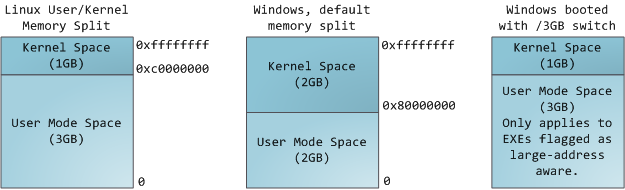
\includegraphics[width=0.8\columnwidth]{kernelUserMemorySplit}
	\captionsource{Répartition de l'espace mémoire du kernel}
	{Répartition de l'espace mémoire virtuel entre le noyau et le programme, par G.~Duarte}
	{\url{http://duartes.org/gustavo/blog/post/anatomy-of-a-program-in-memory/}}
	\label{fig:kernelUserMemorySplit}
\end{figure}

L'espace réserver au programme est ensuite découpé en différents segments tel que la pile (Stack) ou le tas (Heap). Ces segments sont des plages mémoires continues gérées par le système d'exploitation. Dans le cas d'un processus Linux les segments sont réparti ainsi :

\begin{figure}[H]
	\centering
	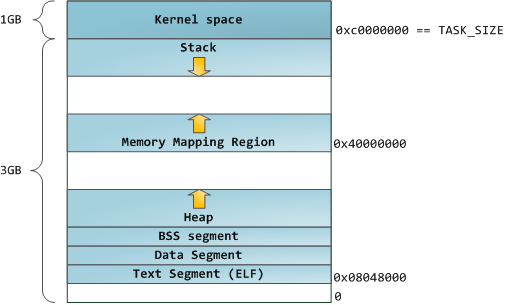
\includegraphics[width=.7\columnwidth]{linuxClassicAddressSpaceLayout}
	\captionsource{Segmentation de la mémoire d'un processus Linux 32 bits}
	{Segmentation de la mémoire d'un processus Linux en 32 bits, par G.~Duarte}
	{\url{http://duartes.org/gustavo/blog/post/anatomy-of-a-program-in-memory/}}
	\label{fig:linuxClassicAddressSpaceLayout}
\end{figure}

La pile d'exécution permet de gérer le flôt de contrôle de l'application. À chaque appel de fonction, une nouvelle structure de pile (Stack frame) est ajoutée à la pile d'exécution et est ensuite retirée lorsque la fonction se termine. La pile d'exécution grandit vers le bas, c'est-à-dire que les adresses mémoires décroissent lorsque la pile se rempli. Il est possible que la pile veuille s'étende au-delà de sa taille maximum, c'est ce que l'on appele un dépassement de pile (Stack overflow) et dans ce cas le programme reçoit une erreur de segmentation (Segmentation fault).

Le segment \og Memory Mapping Region \fg permet au noyau de copier en mémoire le contenu de certains fichiers de manière à augmenter les performances. Ce segment est généralement utilisé pour charger les librairies dynamiques. Il peut aussi être utilisé à d'autres fins, par exemple à la place d'utiliser le tas pour stocker certaines données.

En dessous se trouve le tas, permettant de stocker en mémoire les allocations dynamiques. En C ce segment est géré par la fonction \mintinline{c}|malloc()| et confrères. Dans d'autres langages bénéficiant d'un ramasse miettes tel que le C\#, l'interface pour intéragir avec le tas est le mot reservé \mintinline{c}|new|.

Finalement les trois derniers segments que sont BSS, Data et Text servent a stocker les variables static initialisées ou non ainsi que la source du binaire executé. En \autoref{fig:mappingBinaryImage} un exemple de ce que l'on peut retrouver dans ces segments:

\begin{figure}[H]
	\centering
	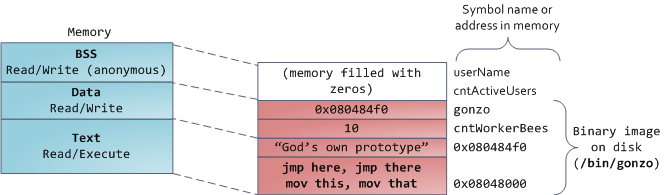
\includegraphics[width=.8\columnwidth]{mappingBinaryImage}
	\captionsource{Mapping d'une image binaire dans les segments BSS, Data et Text}
	{Mapping d'une image binaire dans les segments BSS, Data et Text, par G.~Duarte}
	{\url{http://duartes.org/gustavo/blog/post/anatomy-of-a-program-in-memory/}}
	\label{fig:mappingBinaryImage}
\end{figure}

Lors de l'exécution d'un programme, cette espace virtuel de mémoire est géré par le système d'exploitation grâce à des descripteurs de mémoire (Memory Descriptor). Cette structure contient les adresses de début et de fin de chaque segments.

\begin{figure}[H]
	\centering
	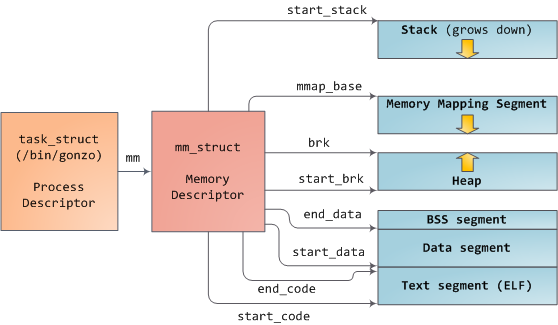
\includegraphics[width=0.6\columnwidth]{mm_struct}
	\captionsource{Descripteur mémoire d'un processus Linux}
	{Descripteur mémoire (Memory Descriptor) d'un processus Linux, par G.~Duarte}
	{\url{http://duartes.org/gustavo/blog/post/how-the-kernel-manages-your-memory/}}
	\label{fig:mm_struct}
\end{figure}

Cette structure est constituée d'une suite de plus petites structures appelées \mintinline{c}{vm_area_struct}. Chacune d'elles est un espace continu en mémoire. Elles permettent de stocker des informations tels que les droits d'écriture et de lecture ou encore les droits d'execution. Elles stockent également si et quel fichier est copié en mémoire.

\begin{figure}[H]
	\centering
	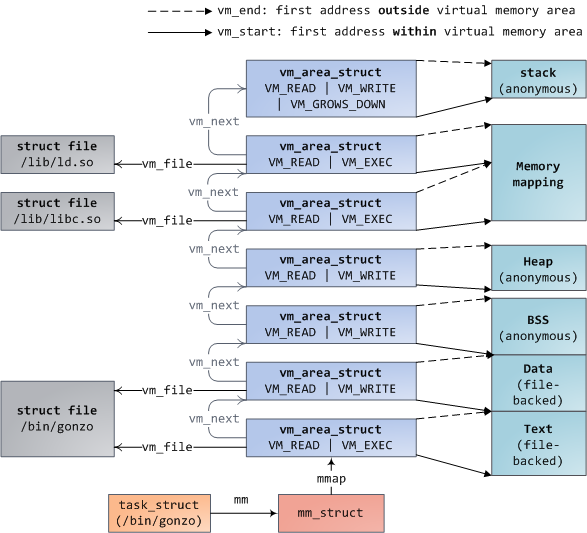
\includegraphics[width=0.9\columnwidth]{memoryDescriptorAndMemoryAreas}
	\captionsource{Structure des espaces virtuels de mémoire (Virtual Memory Area)}
	{Structure des espaces virtuels de mémoire (Virtual Memory Area), par G.~Duarte}
	{\url{http://duartes.org/gustavo/blog/post/how-the-kernel-manages-your-memory/}}
	\label{fig:memoryDescriptorAndMemoryAreas}
\end{figure}

% ---------------------------------------------------------------------------
\section{Buffer overflow}

Le buffer overflow, dépassement de tampon en français, consiste à exploiter une fonction qui ne vérifie par la taille du contenu à copier en mémoire. En utilisant, par exemple, \mintinline{c}{strcpy()}, on peut redéfinir l'adresse de retour de la fonction et ainsi modifier le flôt de contrôle de l'application en le redirigeant à un endroit où l'attaquant aura, par exemple, péalablement injecté son code (p.ex. un shellcode).

Lorsqu'une \og Stack frame \fg est créée, celle-ci stocke dans un schéma particulier les informations d'ont elle a besoin:

\begin{enumerate}
	\item les paramètres passé à la fonction
	\item l'adresse de retour
	\item une sauvegarde du pointeur \mintinline{c}{%ebp}
	\item et les variables locales
\end{enumerate}

Cela permet, en dépassant la taille des variables locales, de modifier des zones mémoires qui ne devraient pas l'être. En regardant la \autoref{fig:stackIntro} on constate que si l'on écrit (8+4+4+4) = 20 octets dans le \mintinline{c}{local_buffer}, les 4 derniers octets auront remplacé l'adresse de retour.

\begin{figure}[H]
	\centering
	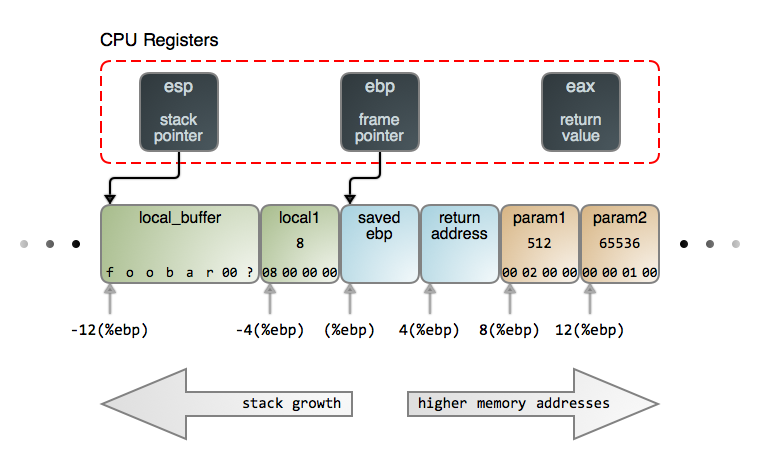
\includegraphics[width=1\columnwidth]{stackIntro}
	\captionsource{Exemple d'une Stack frame}
	{Exemple d'une structure de pile (Stack frame)}
	{\url{http://duartes.org/gustavo/blog/post/journey-to-the-stack/}}
	\label{fig:stackIntro}
\end{figure}

Le code C montré en \autoref{lst:buffer_overflow} illustre un programme vulnérable aux dépassements de tampon en utilisant la fonction \mintinline{c}{strcpy()}. Dans cette exemple trivial il est possible d'injecter un shellcode dans le buffer et de redéfinir l'adresse de retour. On part du principe qu'aucun mécanismes de protection ne sont appliqués à la compilation. La chaîne de caractères copiée dans le \mintinline{c}{local_buffer} est directement contrôlée par l'utilisateur, ce qui rend la manoeuvre encore plus facile.

\begin{listing}
	\cfile{02-main/listings/buffer.c}
	\caption{Exemple de programme vulnérable aux dépassements de tampon}
	\label{lst:buffer_overflow}
\end{listing}

Les mécanismes de protection décrit dans la suite de ce chapitre doivent prévenir l'exploitation de l'exemple montré en \autoref{lst:buffer_overflow} sans obligé le développeur à modifier son code d'une quelconque manière.


\vfill

% ---------------------------------------------------------------------------
\section{DEP/NX}

Pour éviter lors d'un dépassement de tampon que l'attaquant puisse exécuter du code sur la pile. Les endroits mémoire censés contenir des données sont, via les \mintinline{c}{vm_area_struct} sous Linux, marquées comme étant non-executable. Le marquage indique ensuite au processeur, via le \gls{nx} bit, qu'il ne doit pas exécuter le contenu de cette plage mémoire.

\subsection{Mécanisme de protection}

Data Execution Prevention (\gls{dep}) a été introduit sur Linux en 2004 avec la version 2.6.8 du noyau, durant la même année pour Windows et deux ans plus tard pour Mac OS X lors de la transition vers x86 en 2006 \cite{DataExecutionPrevention}.

La protection en soit se base sur le hardware, le NX bit, introduit tout d'abord par AMD en 2003, puis reprise par Intel sous le nom de XD bit une année après \cite{ExecutableSpaceProtection} \cite{NXBit}. Ce bit indique au processeur s'il s'agit d'une zone d'instructions ou de données. Cette fonctionalité hardware peut aussi être simulée, mais cela entraîne de ce fait une baisse de performance importante.

\subsection{Contournements grâce aux attaques \og return-to-libc \fg}

Une pile non-exécutable ne permet plus à l'attaquant d'exécuter son code, mais cela ne l'empêche pas d'exécuter du code marqué comme exécutable déjà présent au sein du programme ou des librairies dynamiquements chargées. Comme montré dans l'exemple de la \autoref{fig:memoryDescriptorAndMemoryAreas}, la bibliothèque partagée \textbf{libc} est chargée en mémoire, ce qui est toujours le cas et ce qui rend une attaque de type \textbf{\og return-to-libc \fg} \cite{ReturntolibcAttack} possible.

Grâce à la fonction \mintinline{c}{system()} présente au sein de \textbf{libc}, il est possible d'exécuter arbitrairement un programme. Lors de l'attaque on localise, par exemple, une chaîne de caractères tel que \mintinline{c}{"/bin/sh"}, que l'on prépare comme étant le paramètre à passer à la fonction \mintinline{c}{system()}.

% ---------------------------------------------------------------------------
\section{ASLR (Address space layout randomization)}

Comme montré sur la \autoref{fig:mappingBinaryImage}, l'espace d'adressage virtuel est structuré de manière fixe. Les emplacements mémoires sont donc inchagés à chaque exécution du programme. De cette manière il est possible de prévoir où se trouve en mémoire les différents composants dont a besoin l'attaque. Une attaque de type \textbf{\og return-to-libc \fg} a besoin de connaître l'adresse de la fonction \mintinline{c}{system()} et de la chaine de caractères \mintinline{c}{"/bin/sh"}. Dans le cas où ces adresses changent à chaque lancement, la tâche devient plus compliquée.

\subsection{Mécanisme de protection}

Depuis juin 2005, l'Address Space Layout Randomization est supportée dans le noyau Linux avec la version 2.6.12 \cite{AddressSpaceLayoutRandomizationFR} \cite{AddressSpaceLayoutRandomizationEN}. Afin de rendre imprédictible les adresses sensibles, trois décalages aléatoires sont effectués au sein de la mémoire virtuelle. Le premier permet de décaler la pile vers le bas, le second décale lui aussi vers le bas le segment de Mapping et le dernier décale vers le haut le segment du tas.

\begin{figure}[H]
	\centering
	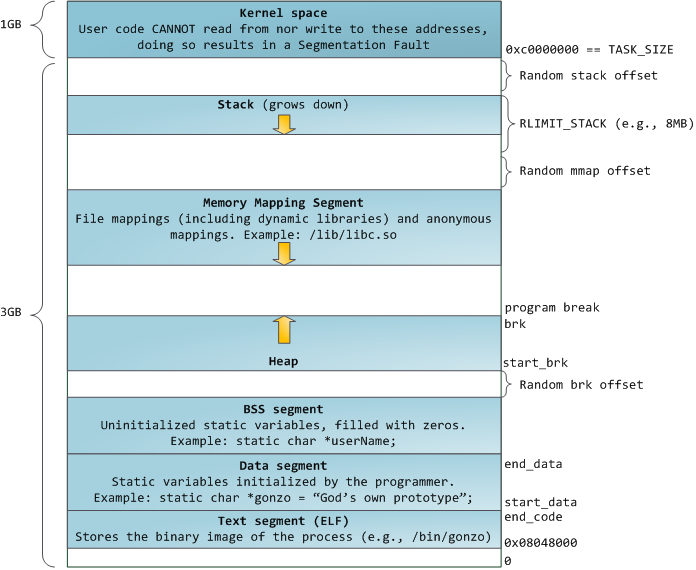
\includegraphics[width=1\columnwidth]{linuxFlexibleAddressSpaceLayout}
	\captionsource{Concept de l'Address space layout randomization sous Linux en 32 bits}
	{Concept de l'Address space layout randomization sous Linux en 32 bits}
	{\url{http://duartes.org/gustavo/blog/post/anatomy-of-a-program-in-memory/}}
	\label{fig:linuxFlexibleAddressSpaceLayout}
\end{figure}

La \autoref{fig:linuxFlexibleAddressSpaceLayout} montre bien qu'en 32~bits, l'espace disponible n'est au total que de 4~Go, la part d'aléatoire est donc restraite. À contrario, dans le cas d'un OS 64~bits ASLR devient bien plus interéssant, car l'espace mémoire virtuel est beaucoup plus vaste (256~To) sans que l'utilisation de celle-ci ne grandisse proportionnellement (au maximum 256~Go de mémoire sont affectés dans des cas classiques d'utilisation serveur). Il donc possible de décaler les segments de manière significative.

Malgré cela, les chercheurs Hector Marco-Gisbert et Ismael Ripoll de l'université de Valence ont écrit un papier démontrant une faiblesse d'\gls{aslr} en 64~bits sous certaines hypothèses \cite{EffectivenessFullASLR64bit}.

\vfill

\subsection{Limitation et contournements}

Sur un OS 32 bits, la marge de manoeuvre laissée au décalage n'est pas très grande. Seule une partie des bits de l'adresse mémoire est utilisée, ce qui laisse possible une attaque de recherche exaustive réussir en quelques milliers d'essais seulement. En effet la pile est placée aléatoirement avec une entropie de 19 bits seulement et le segment de Memory Mapping avec 8 bits.

L'exemple \autoref{lst:bruteforce_aslr} montre comment avec un code python d'une trentaine de lignes il est possible de faire une recherche exhaustive en 32 bits et d'exécuter un shellcode dans un programme n'utilisant pas \gls{dep}/\gls{nx} et les \gls{stackCookies} .

\newpage

\begin{listing}
	\pythonfile{02-main/listings/aslrBruteforce.py}
	\caption{Exemple de recherche exhaustive en python sur ASRL en 32 bits}
	\label{lst:bruteforce_aslr}
\end{listing}

La cas \autoref{lst:bruteforce_aslr} illustre aussi l'utilisation de l'opération \mintinline{python}{"\x90"} indiquant au processeur de passer à l'instruction suivante. En définissant une taile de 4096 bytes de NOP (No Operation) ont augmente drastiquement les chances de tomber sur le shellcode.


% ---------------------------------------------------------------------------
\section{Les stack cannaries}




% ---------------------------------------------------------------------------
\section{Control-Flow integrity}



% \newpage

% % -------------------------------------------------------------------------
% This chapter shows example of picture and also serves to populate the different lists: list of figures, list of tables, bibliography, and glossary.
%
% \section{Tables}
%
% This section contains an examples of table: \autoref{tab:esempio}
%
% \begin{table}[H]
% 	\centering
% 	\begin{tabular}{ccc}
% 		\toprule
% 		name & weight & food \\
% 		\midrule
% 		mouse	& 10 g	& cheese \\
% 		cat	& 1 kg	& mice \\
% 		dog	& 10 kg	& cats \\
% 		t-rex	& 10 Mg	& dogs \\
% 		\bottomrule
% 	\end{tabular}
% 	\caption[A floating table]{A floating table.}
% 	\label{tab:esempio}
% \end{table}
%
% \section{Figures}
%
% This section contains examples of figures: \autoref{fig:galleria}, \autoref{fig:lorem}, \autoref{fig:ipsum}, \autoref{fig:dolor}, \autoref{fig:sit}
%
% \begin{figure}[H]
% 	\centering
% 	\includegraphics[width=0.5\columnwidth]{galleria_stampe}
% 	\captionsource{A floating figure}{A floating figure: the lithograph \emph{Galleria di stampe}, of M.~Escher}{\url{http://www.mcescher.com/}}
% 	\label{fig:galleria}
% \end{figure}
%
% \begin{figure}[H]
% 	\centering
% 	\begin{subfigure}[b]{0.45\textwidth}
% 		\includegraphics[width=\textwidth]{lorem}
% 		\caption{A gull}
% 		\label{fig:lorem}
% 	\end{subfigure}
% 	~ %add desired spacing between images, e. g. ~, \quad, \qquad, \hfill etc.
% 	%(or a blank line to force the subfigure onto a new line)
% 	\begin{subfigure}[b]{0.45\textwidth}
% 		\includegraphics[width=\textwidth]{ipsum}
% 		\caption{A tiger}
% 		\label{fig:ipsum}
% 	\end{subfigure}
% 	~ %add desired spacing between images, e. g. ~, \quad, \qquad, \hfill etc.
% 	%(or a blank line to force the subfigure onto a new line)
% 	\begin{subfigure}[b]{0.45\textwidth}
% 		\includegraphics[width=\textwidth]{dolor}
% 		\caption{A mouse}
% 		\label{fig:dolor}
% 	\end{subfigure}
% 	~ %add desired spacing between images, e. g. ~, \quad, \qquad, \hfill etc.
% 	%(or a blank line to force the subfigure onto a new line)
% 	\begin{subfigure}[b]{0.45\textwidth}
% 		\includegraphics[width=\textwidth]{sit}
% 		\caption{A mouse}
% 		\label{fig:sit}
% 	\end{subfigure}
% 	\caption{Example subcaption}\label{fig:animals}
% \end{figure}
%
%
% % -----------------------------------------------------------------------------
% \section{Code}
%
% \autoref{lst:listing_example} shows an example of Java code rendered with minted.
%
% \begin{listing}
% 	\javafile{02-main/listings/HelloWorld.java}
% 	\caption{Example of listing using the minted package}
% 	\label{lst:listing_example}
% \end{listing}
%
% % -----------------------------------------------------------------------------
% \section{Other features}
%
% Term (glossaries): \gls{nosql}
%
% Acronym (glossaries): \gls{sql}
%
% Citation (biblatex): \cite{paper_millwheel}
%
% % -----------------------------------------------------------------------------
% \section{Conclusion}
%
% \blindtext
